\documentclass[border=10pt]{standalone}
\usepackage{circuitikz}
\usepackage{tikz}
\usetikzlibrary{calc}

\begin{document}
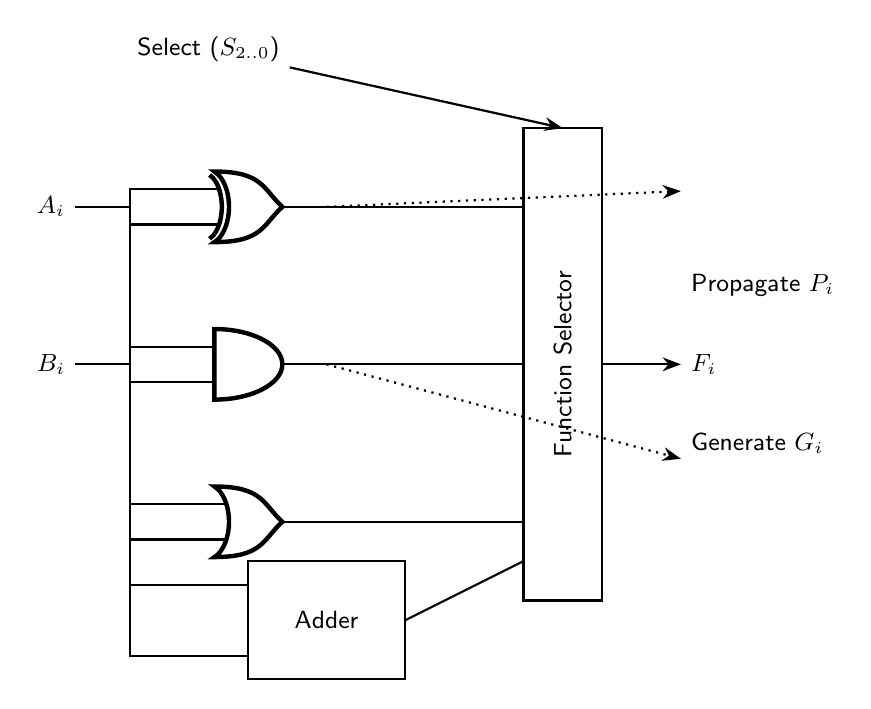
\begin{tikzpicture}[
    >=Stealth, 
    thick, 
    font=\sffamily\small
]

    % Inputs
    \node (Ai) at (0, 6) {$A_i$};
    \node (Bi) at (0, 4) {$B_i$};
    \node (Si) at (2, 8) {Select ($S_{2..0}$)};

    % Logic Gates (Conceptual)
    % We will show a cloud or block for "Logic/Arithmetic Gen"
    % actually 74381 uses a mix of gates. Let's draw a few representative ones feeding a Mux.
    
    % XOR
    \node[american xor port, scale=0.8] (xor) at (3, 6) {};
    % AND
    \node[american and port, scale=0.8] (and) at (3, 4) {};
    % OR
    \node[american or port, scale=0.8] (or) at (3, 2) {};
    
    % Adder (Full Adder)
    \draw[fill=white] (2.5, 0) rectangle (4.5, 1.5);
    \node at (3.5, 0.75) {Adder};

    % Mux
    \draw[fill=white] (6, 1) rectangle (7, 7);
    \node[rotate=90] at (6.5, 4) {Function Selector};
    
    % Connections
    \draw (Ai) -- (1, 6) |- (xor.in 1);
    \draw (1, 6) |- (and.in 1);
    \draw (1, 6) |- (or.in 1);
    \draw (1, 6) |- (2.5, 1.2); % To Adder

    \draw (Bi) -- (1, 4) |- (xor.in 2);
    \draw (1, 4) |- (and.in 2);
    \draw (1, 4) |- (or.in 2);
    \draw (1, 4) |- (2.5, 0.3); % To Adder

    % Gate outputs to Mux
    \draw (xor.out) -- (6, 6);
    \draw (and.out) -- (6, 4);
    \draw (or.out) -- (6, 2);
    \draw (4.5, 0.75) -- (6, 1.5);

    % Select lines
    \draw[->] (Si) -- (6.5, 7);

    % Outputs
    \draw[->] (7, 4) -- (8, 4) node[right] {$F_i$};
    
    % Propagate / Generate from simplified logic
    \node[right] at (8, 5) {Propagate $P_i$};
    \node[right] at (8, 3) {Generate $G_i$};
    
    % Connecting P/G lines conceptually
    \draw[dotted, ->] (3.5, 6) -- (8, 6.2); % From XOR/Logic
    \draw[dotted, ->] (3.5, 4) -- (8, 2.8); % From AND/Logic

\end{tikzpicture}
\end{document}
